L'elettrochimica studia fenomeni elettrici dovuti al passaggio di corrente.

Visto che ragioniamo sempre in soluzioni acquose, il passaggio di corrente provoca dei fenomeni chimici. Può accadere anche il contrario: si genera energia elettrica tramite una reazione. Tratteremo entrambi i casi.

\vspace{0.2cm}Va da ricordare che energia elettrica significa flusso di elettroni.

Le reazioni che comportano scambi di elettroni sono le ossidoriduzioni, pertanto saremo interessati a questo tipo di reazioni.

Le redox a cui siamo interessati devono essere spontanee, perché sennò avverrebbe il contrario: facendo passare la corrente in soluzione indurremo reazioni redox. Dunque qualunque reazione redox spontanea è una sorgente di energia elettrica, ossia possiamo costruire una pila a partire da reazioni redox (tutte le pile comportano reazioni redox).

Consideriamo due esempi:

\begin{figure}[H]
    \centering
    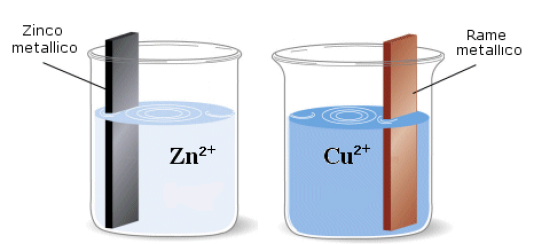
\includegraphics[width=12cm]{immagini/piastre_metalliche.png}
\end{figure}

Consideriamo dei beker conteneti acqua distillata in cui sono immersi un filo di zinco e un filo di rame. Tale sistema è chiamato \textbf{semicella}.

In entrambi i casi stiamo immergendo in acqua un metallo, il quale inizia a liberare ioni. Ne segue che la lamina si caricherà di elettroni lasciati sulla lamina dagli ioni. Quindi la lamina, inizialmente neutra, immersa in acqua si carica negativamete e l'acqua distillata si arricchirà di ioni metallici. Quindi la soluzione inizialmente neutra si caricherà positivamente perché sta accettando cationi, mentre la lamina si caricherà negativamente perché ogni atomo che va in soluzione lascia elettroni su di essa. Poiché la lamina costituisce la parte conduttrice della semicella che estrae o immette corrente elettrica in questa viene chiamato \textbf{elettrodo}.

Si crea quindi un doppio strato elettrico tra soluzione e lamina metallica, rispettivamente cariche positivamente e negativamente, e dunque si forma una differenza di potenziale. Tuttavia non siamo in grado di misurare questa d.d.p. perché per misurarla dovremmo usare un tester con cui tocchiamo la lamina con un puntale e la soluzione con l'altro, ma il puntale immerso in soluzioni libererà ioni caricandosi negativamente. In conseguenza a ciò la d.d.p. letta sarebbe quella tra la lamina e il puntale immerso in soluzione, e non quella tra la lamina e la soluzione.

Come si fa?

Ci si accorge che metalli diversi hanno capacità diverse di liberare ioni in soluzione, cioè ne liberano quantità diverse. Dato che è possibile misurare gli ioni in soluzione in quanto le soluzioni in cui sono presenti ioni conducono e quindi si può misurare il numero di portatori di carica, sappiamo che la lamina di zinco, a parità di condizioni, libera molti più ioni in acqua di quanti non ne liberi la lamina di rame. Se quindi accoppiassimo questi due elettrodi in teoria sarebbero entrambi negativi, nella pratica quella di zinco è molto più negativa di quella di rame, per cui nell'istante in cui accoppiamo le due semicelle e le colleghiamo, convenzionalmente quella più negativa assumerà segno negativo e quella meno negativa segno positivo. Dunque da separati tutti i metalli liberano ioni in soluzione e sono tutti negativi, ma nel momento in cui li accoppiamo quello più negativo tra i due assumerà carica negativa e quello meno negativo carica positiva, perché il flusso di elettroni andrà sempre da quello più negativo a quello meno negativo. In questo caso il flusso di elettroni andrà dallo zinco verso il rame, cioè l'elettrodo del rame sta ricevendo elettroni, per cui sarà positivo.

Quanti elettroni liberano in soluzione?

In realtà pochi, tant'è che quando mettiamo una lamina di un metallo in acqua questa, sebbene inizi a liberare ioni, non si scioglie. Pertanto il numero di ioni liberati è limitato. Ad un certo punto però si raggiunge un equilibrio, ossia gli ioni che sono in soluzione sono positivi, ma la lamina si è caricata negativamente, quindi si genera un campo elettrico che tende a far tornare gli ioni sulla lamina. La lamina però tenderà a liberarli nuovamente, fino a quando si raggiunge un equilibrio dinamico in cui il numero di ioni liberati in soluzione è pari al numero di ioni che dalla soluzione ritornano alla lamina. Quest'equilibrio non si raggiunge velocemente perché in acqua sono presenti anche ioni $\rm H_3O^+$ dovuti all'autodissociazione dell'acqua, i quali sentono anch'essi il campo della lamina e competono con i cationi metallci per raggiungere la lamina, turbando dunque il raggiungimento dell'equilibrio.

Pertanto non è conveniente immergere lamine metalliche in acqua, in quanto difficilmente raggiungeremo un equilibrio, conviene piuttosto immergerle in soluzioni dei loro sali, in modo tale da avere già in soluzione una concentrazione di ioni metallici molto alta, di gran lunga superiore alla concentrazione di $10^{-7}$ ioni $\rm H_3O^+$ per litro dovuti all'autodissociazione dell'acqua in modo da far sì che il turbamento dovuto a tali ioni sia irrilevante poiché la loro quantità è insignificante rispetto a quella degli ioni metallici.

\subsection{Misura della d.d.p. (pila di Daniell)}
\begin{figure}[H]
    \centering
    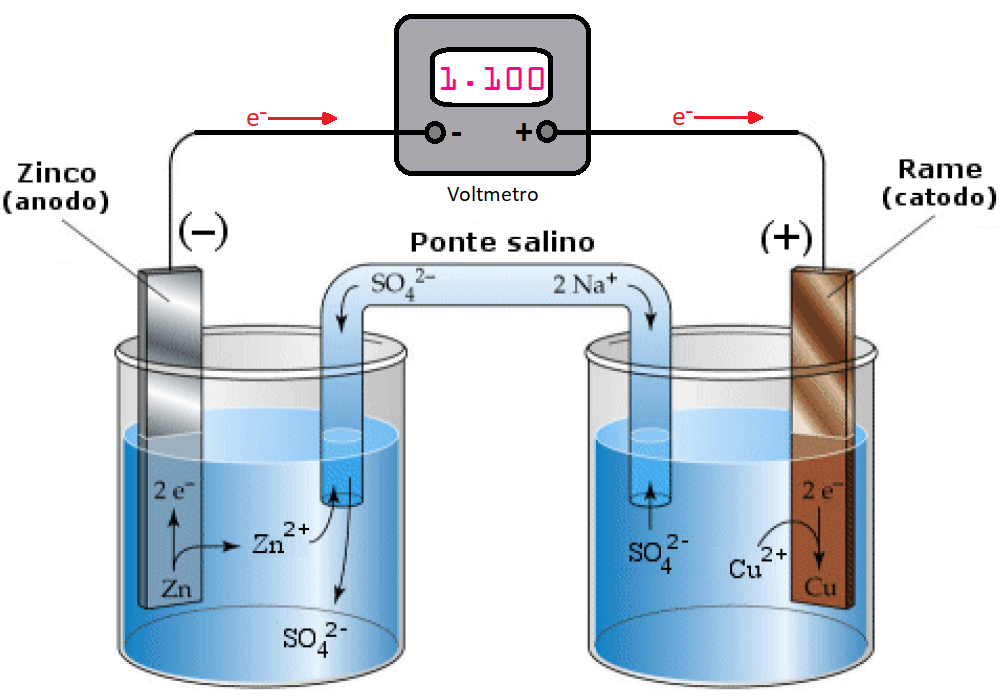
\includegraphics[width=12cm]{immagini/pila_di_Daniell.png}
\end{figure}
\begin{center}
    \hspace{0.3cm}\begin{tabular}{p{3.6cm}p{1.3cm}p{3.8cm}}
    \ce{Zn -> Zn^{2+} + 2 e^-} & & \ce{Cu^{2+} + 2e^- -> Cu}\\
    ossidazione, anodo & & riduzione, catodo
    \end{tabular}
\end{center}

Esso rappresenta il modello di pila più semplice che possiamo immmaginare.

Abbiamo una lamina di zinco immersa in una soluzione di solfato di zinco, in modo tale che quando la lamina libera ioni zinco in soluzione sono già presenti ioni di questo tipo. Ciò che accade è che lo zinco in acqua libera ioni $\rm Zn^{2+}$ e lascia due elettroni per atomo sulla lamina, che si carica negativamente.

Abbiamo poi una lamina di rame, la quale in teoria libera ioni $\rm Cu^{2+}$. Per lo stesso motivo della lamina di zinco è immersa in una soluzione di solfato di rame in cui tali ioni sono già presenti così che l'equilibrio si instauri velocemente.

Colleghiamo i due elettrodi. Sapendo che la lamina di zinco si carica più negativamente della lamina di rame perché libera in soluzione molti più ioni ioni zinco di quanti ioni rame libera in soluzione la lamina di rame, di conseguenza ci saranno più elettroni sulla lamina di zinco che su quella di rame e quindi gli elettroni fluiranno dalla prima alla seconda.

Per chiudere il circuito però dobbiamo collegare anche le soluzioni. Infatti nelle condizioni in cui di trova adesso
il sistema
$$(-) \; \ce{Zn <--> Zn^{2+}(aq) + 2e^-} \qquad (+) \; \ce{ Cu^{2+}(aq) + 2e^- <--> Cu}$$

Quindi su un elettrodo abbiamo l'ossidazione dello zinco, sull'altro la riduzione del rame. Cosa succede alle soluzioni appena avviene ciò?

A sinistra arrivano ioni zinco, e la soluzione inizialmente neutra a causa degli ioni $\rm Zn^{2+}$

$$\ce{Zn + Cu^{2+}(aq) <--> Zn^{2+}(aq) + Cu}$$

$$L_{\text{utile}}=- \Delta G; \; L_{\text{utile}}=L_{\text{elettrico}}=q_c \times E=nFE$$

$$\implies \Delta G = -nFE$$

$$\ce{\alpha A + \beta B <--> \gamma C + \delta D}$$

$$\Delta G = \Delta G^0 + RT\ln k \quad \text{con }k \text{ costante di equilibrio}$$

$$\Delta G=0 \implies \Delta G^0= -RT \ln k$$

$$\Delta G =  -RT \ln k_{eq} + RT \ln \frac{a_C^{\gamma} \, a_D^{\delta}}{a_A^{\alpha} \, a_B^{\beta}}=-nFE$$

$$E=\frac{RT}{nF}\ln k_{eq} - \frac{RT}{nF}\ln \frac{a_C^{\gamma} \, a_D^{\delta}}{a_A^{\alpha} \, a_B^{\beta}}$$

$$E= E_0 + \frac{RT}{nF}\ln \frac{a_C^{\gamma} \, a_D^{\delta}}{a_A^{\alpha} \, a_B^{\beta}} \quad \textbf{Equazione di Nerst}$$

Se poniamo

$$R=8.314 \, J/mol\,K, \quad \ln x = 2.303 \log x, \quad F=96483 \, C, \quad T=298 \,K$$

L'equazione diventa

$$E = E_0 + \frac{0.059}{n}\log \frac{a_C^{\gamma} \, a_D^{\delta}}{a_A^{\alpha} \, a_B^{\beta}}$$

$n$ resta tale perché dipende da quanti elettroni genera quella reazione.

\vspace{0.2cm}Per un generico elettrodo vale

$$\ce{\alpha M^{n+} + ne^- <--> \beta M}$$

$$E = E_0 + \frac{0.059}{n}\log \frac{a_{ox}^{\alpha}}{a_{rid}^{\beta}}$$

$$E = E_0 + \frac{0.059}{n}\log a(\text{Mn}^+)^{\alpha}$$